\ifdefined\included
\else
\setcounter{chapter}{2} %% Numéro du chapitre précédent ;)
\dominitoc
\faketableofcontents
\fi

\chapter{Ontologenius: A long-term semantic memory}
\minitoc

\section{Design and features}

\subsection{Why an ontology?}

\subsection{Ontology formalism}

Even if we saw that the use of ontology is today a common way to represent semantic knowledge, we will recall in this subsection the composition of an ontology. For each element composing it, we will draw a formalization then give examples using the Turtle syntax. The pieces of ontologies used in the examples of this subsection are voluntarily simplified. The introduced notations will be the ones used in the rest of this thesis and the graphical representations, both in terms of color and form, will be kept as often as possible.

On the base of the definition of a Description Logic ontology presneted in \cite{fokoue_2006_summary}, we define a semantic knowledge base $\kbs$ represented as an ontology by  $\kbs = \langle \Abox, \Tbox, \Rbox \rangle$. $\Abox$, $\Tbox$, and $\Rbox$ are respectively called the Abox, Tbox, and Rbox of the ontology.


\begin{figure}[h!]
\centering
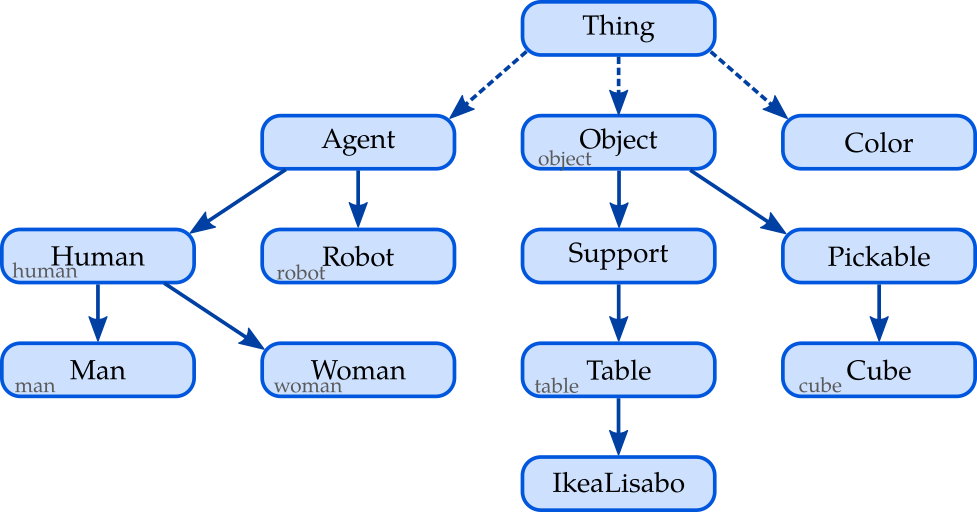
\includegraphics[scale=0.4]{figures/chapter2/Tbox.png}
\caption{\label{fig:Tbox} Representation of an ontology class hierarchy graph to illustrate the composition of a TBox. Taking the class Human, the bottom arrow has to be read as \textit{"A man is a kind of Human"}. The texts at the bottom left of the class, if there is, are the classes' labels in natural language.}
\end{figure}

The Tbox $\Tbox$ contains assertions about the classes (types) of the ontology. It is defined by $\Tbox = \langle \classset, H \rangle$. It can be see as a directed acyclic graph as presented in Figure~\ref{fig:Tbox}. $\classset$ is the set of all the classes of the ontology. In our example, $\classset = \{Thing,\ Agent,\ Object, ...,\ IkeaLisabo\}$. Considering the Tbox as a graph, $H$ stores its directed edges. It represents the inheritance links between the classes (i.e. the subsumption assertions). This link is commonly referred as the "isA" link (e.g. \textit{(Human, isA, Agent)}) and is described with the property rdfs:subClassOf in the OWL language as illustrated in the Listing~\ref{lst:Tbox}.

\begin{lstlisting}[frame=single, basicstyle=\scriptsize\ttfamily, label={lst:Tbox}, caption={Description of ontology classes in the OWL language using the Turle syntax.},captionpos=b]
:Human rdf:type owl:Class ;
       rdfs:subClassOf :Agent .

:Man   rdf:type owl:Class ;
       rdfs:subClassOf :Human .
\end{lstlisting}

\begin{figure}[h!]
\centering
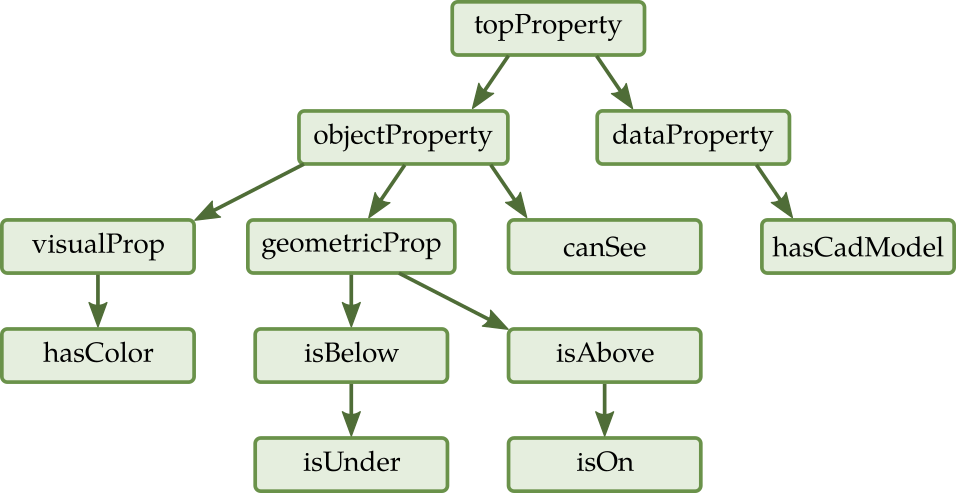
\includegraphics[scale=0.4]{figures/chapter2/Rbox.png}
\caption{\label{fig:Rbox} Representation of an ontology property hierarchy graph to illustrate the composition of an RBox. Taking the property isBelow, the bottom arrow has to be read as: \textit{"The property isUnder is a specification of the property isBelow"}.}
\end{figure}

The Rbox $\Rbox$ contains assertions about the properties (roles). It is at least defined by the $\Rbox = \langle \propset, \inclset, \invset, \domainset, \rangeset \rangle$. In the same way of the Tbox, $\propset$ is the set of properties and $\inclset$ stores the directed edges of the finite directed acyclic graph representing the inheritance links between the properties. Such a graph is represneted in Figure~\ref{fig:Rbox}. These inheritance links aim at specifying properties. On our example, the property IsOn is a specification of the property isAbove in the way that an object being on another is an object that is above the latter and being in contact with. It is described with the property rdfs:subPropertyOf in the OWL language. 
$Inv = \{(\property, \property^{-1}) \in \propset^2\}$ is the set representing the properties inverses (\textit{e.g.} $(isOn, isUnder) \in Inv$). Describing the inverse of a property is useful first to reduce description work since if some describe a relation involving a property for which an inverse is define, the inverse relation is also describe in an underlying way. Moreover, for an algorithm exploring an ontology, knowing that a relation use a property having an inverse can allow to reduce the algorithm complexity by not concidering the inverse relation into the exploration.
Finally, $\domainset$ and $\rangeset$ are respectively 


Finally, the ABox $\Abox = \langle \indivset, \inheritset_0, \relationset \rangle$, with $\indivset$ the set of individuals/entities, $\inheritset_0$ the set of direct types of $\indivset$ such as $\inheritset_0 = \{(\indiv, \class) | \indiv \in \indivset, \class \in \classset \}$ (an instance $\indiv$ can have several direct types) and $\relationset$ the set of relations between entities (i.e. the triplets) such as $\relationset = \{(\subject, \property ,\object) | (\subject, \object) \in \indivset^2, \property \in \propset\}$ where $\subject$ is the subject, $\property$ the property and $\object$ the object. With theses relations we can both represent the attributes of an entity but also represent relations between entities such as spatial relations relating to other entities.


While $\inheritset_0$ contains the direct types of entities, we use $\inheritset$ to denote set of direct and inherited types.
For instance, an entity \textit{dog23} with a direct \textit{Dog} type ($(dog23, Dog) \in \inheritset_0$) would also inherit the \textit{Animal} type ($(dog23, Dog), (dog23, Animal) \in \inheritset$) through the type hierarchy of $\Tbox$. When appropriate, the REG will take benefit of this  inheritance to refer to entities with a higher level of abstraction.

Note that to fully match the Fokue definition \cite{hutchison_summary_2006}, we also need to add the disjunctive, transitive, reflexive and chain relations declarations in $\Rbox$ and disjunctive class declarations in $\Tbox$. Since we will not use them in here we chose to not take them into account in this definition. We also assume that all inference processes have already been made resulting in complete and consistent knowledge base to be used by the REG.

\begin{figure}[h!]
\centering
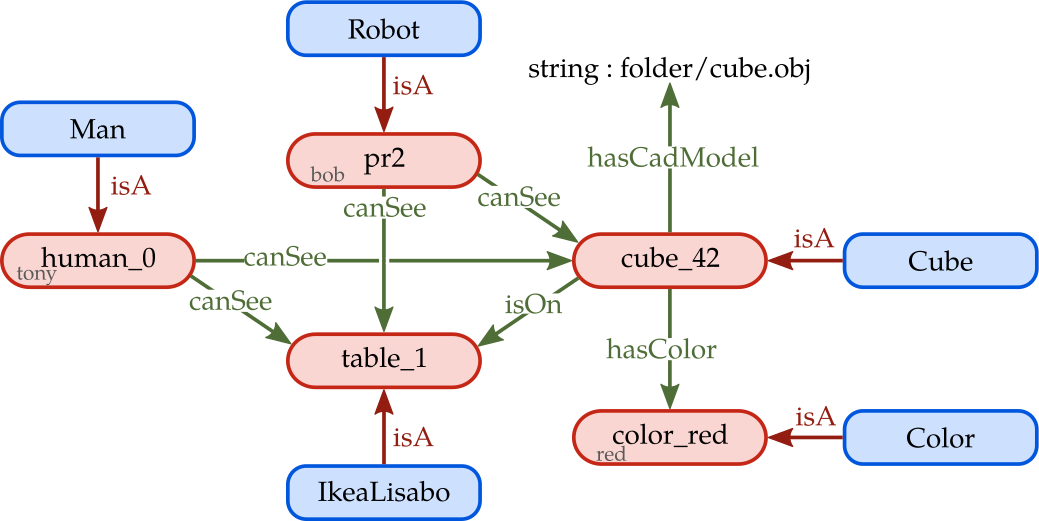
\includegraphics[scale=0.4]{figures/chapter2/Abox.png}
\caption{\label{fig:Abox}  Representation of an ontology instances graph to illustrate the composition of an ABox. Red boxes are individuals of the ontology. Green arrows are properties coming from the RBox and applied to individuals. Red arrows represent a direct inheritance link between an individual and a class coming from the TBox. The texts at the bottom left of the individuals, if there is, are the individuals' labels in natural language.}
\end{figure}

\subsection{Desired features}


\section{Architecture}

\subsection{Permanent versus temporary data structure}

\subsection{Concepts' identifier versus name in natural language}

\subsection{Resoning to enrich the knowledge}



\section{Managing others' estimated knowledge}

\subsection{Ontologenius multi-instances principle}

\subsection{Catching knowledge at a given moment}

\subsection{Exploring several possible mental states at once}



\section{Using Ontologenius in robotic applications}

\subsection{Inserting new knowledge}

\subsection{Retrieving knowledge}

\subsubsection{Low-level queries}

\subsubsection{SPARQL-like interface}

\subsection{The Application Programming Interface}

\subsubsection{Debbuging tool}



\section{Computational preformance evaluation}

\subsection{Concepts recovery}

\subsection{Low-level queries}

\subsection{SPAQRL queries}

Lorem ipsum dolor sit amet, consectetur adipiscing elit. Sed non risus. Suspendisse lectus tortor, dignissim sit amet, adipiscing nec, ultricies sed, dolor. Cras elementum ultrices diam. Maecenas ligula massa, varius a, semper congue, euismod non, mi. Proin porttitor, orci nec nonummy molestie, enim est eleifend mi, non fermentum diam nisl sit amet erat. Duis semper. Duis arcu massa, scelerisque vitae, consequat in, pretium a, enim. Pellentesque congue. Ut in risus volutpat libero pharetra tempor. Cras vestibulum bibendum augue. Praesent egestas leo in pede. Praesent blandit odio eu enim. Pellentesque sed dui ut augue blandit sodales. Vestibulum ante ipsum primis in faucibus orci luctus et ultrices posuere cubilia Curae; Aliquam nibh. Mauris ac mauris sed pede pellentesque fermentum. Maecenas adipiscing ante non diam sodales hendrerit.

Ut velit mauris, egestas sed, gravida nec, ornare ut, mi. Aenean ut orci vel massa suscipit pulvinar. Nulla sollicitudin. Fusce varius, ligula non tempus aliquam, nunc turpis ullamcorper nibh, in tempus sapien eros vitae ligula. Pellentesque rhoncus nunc et augue. Integer id felis. Curabitur aliquet pellentesque diam. Integer quis metus vitae elit lobortis egestas. Lorem ipsum dolor sit amet, consectetuer adipiscing elit. Morbi vel erat non mauris convallis vehicula. Nulla et sapien. Integer tortor tellus, aliquam faucibus, convallis id, congue eu, quam. Mauris ullamcorper felis vitae erat. Proin feugiat, augue non elementum posuere, metus purus iaculis lectus, et tristique ligula justo vitae magna.
Aliquam convallis sollicitudin purus. Praesent aliquam, enim at fermentum mollis, ligula massa adipiscing nisl, ac euismod nibh nisl eu lectus. Fusce vulputate sem at sapien. Vivamus leo. Aliquam euismod libero eu enim. Nulla nec felis sed leo placerat imperdiet. Aenean suscipit nulla in justo. Suspendisse cursus rutrum augue. Nulla tincidunt tincidunt mi. Curabitur iaculis, lorem vel rhoncus faucibus, felis magna fermentum augue, et ultricies lacus lorem varius purus. Curabitur eu amet.

